\documentclass{article}
\usepackage{amsmath}
\usepackage{amssymb}
\usepackage{graphicx}
\usepackage{enumitem}
\usepackage[utf8]{inputenc}
\graphicspath{{/home/stephanie/Escritorio/THC/Taller-de-Herramientas-Computacionales/Clases/Latex/Imagenes/}}

\title{\Huge Taller de Herramientas Computacionales}
\author{Stephanie Escobar Sánchez}
\date{15/enero/2019}
\begin{document}
	\maketitle
\begin{center}
	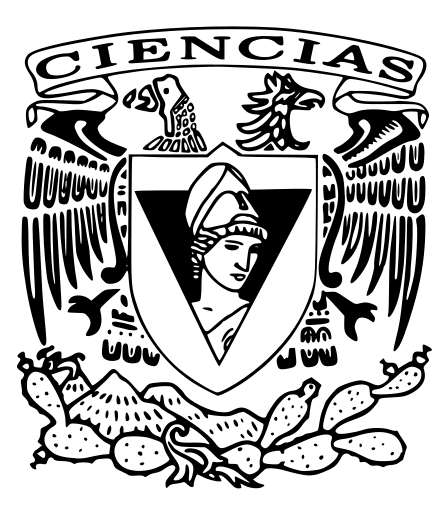
\includegraphics[scale=0.40]{1.png}	
\end{center}
\newpage

%\section{Expresiones Matemáticas}
\section*{Expresiones Matemáticas}
$\alpha + \beta$ %pone la expresión en el centro\\
\[\alpha + \beta\]
\section*{índices y subindices}
$x_{2}$
$x^{2}$\\
\section*{Fracciones}
$\frac{1}{2}$\\
$\frac{\frac{3}{4}1}{\frac{3}{5}}$\\
$\sqrt{2} + \sqrt{3^2}^2$\\
\%\\ %Para que reconozca el simbolo
$\int_{a}^{b} x^2 dx$\\
$\int_{a}^{b} x^2 \partial x^2$\\
$3 \quad 2$
%\dots puntos suspensivos
%\vdots puntos suspensivos verticales
\section{Matrices}
\[
\begin{bmatrix}
x_{2} & x_3\\
x_{4} & x_6	
\end{bmatrix}
\] %los corchetes son como pesitos pero para centrarlo
\[
\begin{bmatrix}
x_{2} & x_{3} & \dots
\vdots & \dots & \dots

\end{bmatrix}
\]
$\sum$
\end{document}